\subsection{Tables and figures}

Table~\ref{tab:best-models} summarizes the strongest mean model performance for each dataset and metric. Table~\ref{tab:paired-statistics} reports the paired TabPFN-versus-tree comparisons, while Table~\ref{tab:model-summary} provides the model-level aggregate F1 and ROC-AUC results. Table~\ref{tab:training-regimes} presents the ROC-AUC comparisons by training-data regime. Training and prediction times are reported separately in Table~\ref{tab:computational-performance}.

\begin{longtable}{llLNN}
\caption{Best mean performance by dataset and metric.}\label{tab:best-models}\\
\toprule
Dataset & Metric & Best model & Mean & Std \\
\midrule
\endfirsthead
\toprule
Dataset & Metric & Best model & Mean & Std \\
\midrule
\endhead
Adult & Accuracy & CatBoost & 0.8409 & 0.0340 \\
Adult & Precision & CatBoost & 0.7330 & 0.0897 \\
Adult & Recall & XGBoost & 0.5334 & 0.1701 \\
Adult & F1 & CatBoost & 0.5936 & 0.1509 \\
Adult & ROC\_AUC & CatBoost & 0.8787 & 0.0650 \\
Bank Marketing & Accuracy & TabPFN & 0.8980 & 0.0137 \\
Bank Marketing & Precision & CatBoost & 0.6022 & 0.1171 \\
Bank Marketing & Recall & TabPFN & 0.3201 & 0.1924 \\
Bank Marketing & F1 & TabPFN & 0.3860 & 0.2046 \\
Bank Marketing & ROC\_AUC & TabPFN & 0.8716 & 0.0939 \\
Credit-G & Accuracy & CatBoost & 0.7212 & 0.0296 \\
Credit-G & Precision & XGBoost & 0.7621 & 0.0357 \\
Credit-G & Recall & CatBoost & 0.8957 & 0.0338 \\
Credit-G & F1 & CatBoost & 0.8182 & 0.0181 \\
Credit-G & ROC\_AUC & CatBoost & 0.7213 & 0.0557 \\
\bottomrule
\end{longtable}

\begingroup
\footnotesize
\setlength{\tabcolsep}{2pt}
\renewcommand{\arraystretch}{1.05}
\begin{longtable}{p{2.6cm}p{1.75cm}p{1.55cm}R{1.1cm}R{1.7cm}R{1.4cm}p{2.2cm}p{1.75cm}}
\caption{Paired statistical comparison of TabPFN against gradient-boosted tree models. Difference is TabPFN minus the tree-model mean.}\label{tab:paired-statistics}\\
\toprule
Dataset & Metric & Tree & $\Delta$ & $p$ (unadjusted) & $p$ (Holm) & Direction & Holm significant \\
\midrule
\endfirsthead
\toprule
Dataset & Metric & Tree & $\Delta$ & $p$ (unadjusted) & $p$ (Holm) & Direction & Holm significant \\
\midrule
\endhead
Adult & Accuracy & XGBoost & 0.0097 & <0.0001 & <0.0001 & TabPFN higher & Yes \\
Adult & Accuracy & LightGBM & 0.0100 & <0.0001 & 1.00e-05 & TabPFN higher & Yes \\
Adult & Accuracy & CatBoost & -0.0059 & <0.0001 & <0.0001 & TabPFN lower & Yes \\
Adult & Precision & XGBoost & 0.0665 & <0.0001 & <0.0001 & TabPFN higher & Yes \\
Adult & Precision & LightGBM & 0.1141 & <0.0001 & <0.0001 & TabPFN higher & Yes \\
Adult & Precision & CatBoost & -0.0300 & <0.0001 & <0.0001 & TabPFN lower & Yes \\
Adult & Recall & XGBoost & -0.0096 & 0.0031 & 0.0470 & TabPFN lower & Yes \\
Adult & Recall & LightGBM & 0.0276 & 0.7248 & 1.0000 & TabPFN higher & No \\
Adult & Recall & CatBoost & 0.0044 & 0.6499 & 1.0000 & TabPFN higher & No \\
Adult & F1 & XGBoost & 0.0094 & 0.0112 & 0.1346 & TabPFN higher & No \\
Adult & F1 & LightGBM & 0.0477 & 0.0002 & 0.0043 & TabPFN higher & Yes \\
Adult & F1 & CatBoost & -0.0098 & 0.0002 & 0.0035 & TabPFN lower & Yes \\
Adult & ROC\_AUC & XGBoost & 0.0280 & <0.0001 & <0.0001 & TabPFN higher & Yes \\
Adult & ROC\_AUC & LightGBM & 0.0521 & <0.0001 & <0.0001 & TabPFN higher & Yes \\
Adult & ROC\_AUC & CatBoost & -0.0043 & 7.00e-05 & 0.0015 & TabPFN lower & Yes \\
Bank Marketing & Accuracy & XGBoost & 0.0106 & <0.0001 & <0.0001 & TabPFN higher & Yes \\
Bank Marketing & Accuracy & LightGBM & 0.0092 & <0.0001 & <0.0001 & TabPFN higher & Yes \\
Bank Marketing & Accuracy & CatBoost & 0.0012 & <0.0001 & 1.00e-05 & TabPFN higher & Yes \\
Bank Marketing & Precision & XGBoost & 0.0985 & <0.0001 & <0.0001 & TabPFN higher & Yes \\
Bank Marketing & Precision & LightGBM & 0.1109 & <0.0001 & <0.0001 & TabPFN higher & Yes \\
Bank Marketing & Precision & CatBoost & -0.0361 & 0.8693 & 1.0000 & TabPFN lower & No \\
Bank Marketing & Recall & XGBoost & 0.0156 & 0.0009 & 0.0141 & TabPFN higher & Yes \\
Bank Marketing & Recall & LightGBM & 0.0341 & <0.0001 & <0.0001 & TabPFN higher & Yes \\
Bank Marketing & Recall & CatBoost & 0.0480 & <0.0001 & <0.0001 & TabPFN higher & Yes \\
Bank Marketing & F1 & XGBoost & 0.0215 & 1.00e-05 & 0.0002 & TabPFN higher & Yes \\
Bank Marketing & F1 & LightGBM & 0.0382 & <0.0001 & <0.0001 & TabPFN higher & Yes \\
Bank Marketing & F1 & CatBoost & 0.0396 & <0.0001 & <0.0001 & TabPFN higher & Yes \\
Bank Marketing & ROC\_AUC & XGBoost & 0.0571 & <0.0001 & <0.0001 & TabPFN higher & Yes \\
Bank Marketing & ROC\_AUC & LightGBM & 0.0601 & <0.0001 & <0.0001 & TabPFN higher & Yes \\
Bank Marketing & ROC\_AUC & CatBoost & 0.0135 & <0.0001 & <0.0001 & TabPFN higher & Yes \\
Credit-G & Accuracy & XGBoost & 0.0170 & 0.0004 & 0.0069 & TabPFN higher & Yes \\
Credit-G & Accuracy & LightGBM & 0.0105 & 0.0061 & 0.0851 & TabPFN higher & No \\
Credit-G & Accuracy & CatBoost & -0.0067 & 0.2069 & 1.0000 & TabPFN lower & No \\
Credit-G & Precision & XGBoost & -0.0070 & 0.1018 & 1.0000 & TabPFN lower & No \\
Credit-G & Precision & LightGBM & 0.0018 & 0.4525 & 1.0000 & TabPFN higher & No \\
Credit-G & Precision & CatBoost & 0.0009 & 0.8184 & 1.0000 & TabPFN higher & No \\
Credit-G & Recall & XGBoost & 0.0539 & <0.0001 & 8.00e-05 & TabPFN higher & Yes \\
Credit-G & Recall & LightGBM & 0.0141 & 0.0965 & 1.0000 & TabPFN higher & No \\
Credit-G & Recall & CatBoost & -0.0099 & 0.2422 & 1.0000 & TabPFN lower & No \\
Credit-G & F1 & XGBoost & 0.0195 & 1.00e-05 & 0.0002 & TabPFN higher & Yes \\
Credit-G & F1 & LightGBM & 0.0091 & 0.0092 & 0.1201 & TabPFN higher & No \\
Credit-G & F1 & CatBoost & -0.0055 & 0.2335 & 1.0000 & TabPFN lower & No \\
Credit-G & ROC\_AUC & XGBoost & 0.0403 & <0.0001 & <0.0001 & TabPFN higher & Yes \\
Credit-G & ROC\_AUC & LightGBM & 0.0748 & <0.0001 & <0.0001 & TabPFN higher & Yes \\
Credit-G & ROC\_AUC & CatBoost & -0.0067 & 0.4780 & 1.0000 & TabPFN lower & No \\
\bottomrule
\end{longtable}
\endgroup

\begin{longtable}{llcNNN}
\caption{Model-level aggregate performance for F1 and ROC-AUC (mean $\pm$ standard deviation).}\label{tab:model-summary}\\
\toprule
Dataset & Model & Metric & $n$ & Mean & Std \\
\midrule
\endfirsthead
\toprule
Dataset & Model & Metric & $n$ & Mean & Std \\
\midrule
\endhead
Adult & CatBoost & F1 & 105 & 0.5936 & 0.1509 \\
Adult & CatBoost & ROC-AUC & 105 & 0.8787 & 0.0650 \\
Adult & LightGBM & F1 & 105 & 0.5361 & 0.2342 \\
Adult & LightGBM & ROC-AUC & 105 & 0.8223 & 0.1413 \\
Adult & TabPFN & F1 & 105 & 0.5838 & 0.1664 \\
Adult & TabPFN & ROC-AUC & 105 & 0.8744 & 0.0675 \\
Adult & XGBoost & F1 & 105 & 0.5744 & 0.1688 \\
Adult & XGBoost & ROC-AUC & 105 & 0.8463 & 0.0987 \\
Bank Marketing & CatBoost & F1 & 105 & 0.3464 & 0.1943 \\
Bank Marketing & CatBoost & ROC-AUC & 105 & 0.8581 & 0.0931 \\
Bank Marketing & LightGBM & F1 & 105 & 0.3479 & 0.1835 \\
Bank Marketing & LightGBM & ROC-AUC & 105 & 0.8115 & 0.1430 \\
Bank Marketing & TabPFN & F1 & 105 & 0.3860 & 0.2046 \\
Bank Marketing & TabPFN & ROC-AUC & 105 & 0.8716 & 0.0939 \\
Bank Marketing & XGBoost & F1 & 105 & 0.3645 & 0.1670 \\
Bank Marketing & XGBoost & ROC-AUC & 105 & 0.8145 & 0.1305 \\
Credit-G & CatBoost & F1 & 50 & 0.8182 & 0.0181 \\
Credit-G & CatBoost & ROC-AUC & 50 & 0.7213 & 0.0557 \\
Credit-G & LightGBM & F1 & 50 & 0.8036 & 0.0256 \\
Credit-G & LightGBM & ROC-AUC & 50 & 0.6398 & 0.1025 \\
Credit-G & TabPFN & F1 & 50 & 0.8126 & 0.0192 \\
Credit-G & TabPFN & ROC-AUC & 50 & 0.7146 & 0.0639 \\
Credit-G & XGBoost & F1 & 50 & 0.7931 & 0.0274 \\
Credit-G & XGBoost & ROC-AUC & 50 & 0.6742 & 0.0710 \\
\bottomrule
\end{longtable}

\begingroup
\footnotesize
\setlength{\tabcolsep}{2.5pt}
\renewcommand{\arraystretch}{1.02}
\begin{longtable}{p{2.35cm}p{1.9cm}p{3.3cm}R{0.55cm}R{1.25cm}R{1.15cm}R{1.15cm}}
\caption{Training-regime comparisons for ROC-AUC. Difference is TabPFN minus the tree-model mean.}\label{tab:training-regimes}\\
\toprule
Dataset & Training regime & Model comparison & $n$ & TabPFN & Tree & $\Delta$ \\
\midrule
\endfirsthead
\toprule
Dataset & Training regime & Model comparison & $n$ & TabPFN & Tree & $\Delta$ \\
\midrule
\endhead
Adult & Small & TabPFN vs XGBoost & 30 & 0.7993 & 0.7304 & 0.0689 \\
Adult & Small & TabPFN vs LightGBM & 30 & 0.7993 & 0.6419 & 0.1574 \\
Adult & Small & TabPFN vs CatBoost & 30 & 0.7993 & 0.8015 & -0.0023 \\
Adult & Medium & TabPFN vs XGBoost & 25 & 0.8900 & 0.8629 & 0.0271 \\
Adult & Medium & TabPFN vs LightGBM & 25 & 0.8900 & 0.8589 & 0.0311 \\
Adult & Medium & TabPFN vs CatBoost & 25 & 0.8900 & 0.8922 & -0.0022 \\
Adult & Large & TabPFN vs XGBoost & 50 & 0.9116 & 0.9076 & 0.0040 \\
Adult & Large & TabPFN vs LightGBM & 50 & 0.9116 & 0.9123 & -0.0006 \\
Adult & Large & TabPFN vs CatBoost & 50 & 0.9116 & 0.9182 & -0.0066 \\
Bank Marketing & Small & TabPFN vs XGBoost & 30 & 0.7520 & 0.6437 & 0.1083 \\
Bank Marketing & Small & TabPFN vs LightGBM & 30 & 0.7520 & 0.6195 & 0.1325 \\
Bank Marketing & Small & TabPFN vs CatBoost & 30 & 0.7520 & 0.7326 & 0.0194 \\
Bank Marketing & Medium & TabPFN vs XGBoost & 25 & 0.8907 & 0.8364 & 0.0543 \\
Bank Marketing & Medium & TabPFN vs LightGBM & 25 & 0.8907 & 0.8388 & 0.0519 \\
Bank Marketing & Medium & TabPFN vs CatBoost & 25 & 0.8907 & 0.8800 & 0.0107 \\
Bank Marketing & Large & TabPFN vs XGBoost & 50 & 0.9339 & 0.9060 & 0.0279 \\
Bank Marketing & Large & TabPFN vs LightGBM & 50 & 0.9339 & 0.9131 & 0.0208 \\
Bank Marketing & Large & TabPFN vs CatBoost & 50 & 0.9339 & 0.9225 & 0.0114 \\
Credit-G & Small & TabPFN vs XGBoost & 30 & 0.6767 & 0.6376 & 0.0391 \\
Credit-G & Small & TabPFN vs LightGBM & 30 & 0.6767 & 0.5814 & 0.0953 \\
Credit-G & Small & TabPFN vs CatBoost & 30 & 0.6767 & 0.6922 & -0.0155 \\
Credit-G & Medium & TabPFN vs XGBoost & 20 & 0.7714 & 0.7292 & 0.0422 \\
Credit-G & Medium & TabPFN vs LightGBM & 20 & 0.7714 & 0.7273 & 0.0441 \\
Credit-G & Medium & TabPFN vs CatBoost & 20 & 0.7714 & 0.7651 & 0.0063 \\
\bottomrule
\end{longtable}
\endgroup

\begin{longtable}{llNNNN}
\caption{Mean computational measurements in seconds, reported separately for training and prediction.}\label{tab:computational-performance}\\
\toprule
Dataset & Model & Training Mean & Training Std & Prediction Mean & Prediction Std \\
\midrule
\endfirsthead
\toprule
Dataset & Model & Training Mean & Training Std & Prediction Mean & Prediction Std \\
\midrule
\endhead
Adult & CatBoost & 0.558 & 0.391 & 0.049 & 0.004 \\
Adult & LightGBM & 0.189 & 0.170 & 0.099 & 0.033 \\
Adult & TabPFN & 0.679 & 0.074 & 9.036 & 13.622 \\
Adult & XGBoost & 0.174 & 0.154 & 0.062 & 0.009 \\
Bank Marketing & CatBoost & 0.625 & 0.391 & 0.042 & 0.003 \\
Bank Marketing & LightGBM & 0.205 & 0.182 & 0.091 & 0.030 \\
Bank Marketing & TabPFN & 0.685 & 0.074 & 8.946 & 13.517 \\
Bank Marketing & XGBoost & 0.212 & 0.216 & 0.046 & 0.005 \\
Credit-G & CatBoost & 0.351 & 0.037 & 0.011 & 0.002 \\
Credit-G & LightGBM & 0.052 & 0.048 & 0.011 & 0.001 \\
Credit-G & TabPFN & 0.659 & 0.059 & 0.667 & 0.016 \\
Credit-G & XGBoost & 0.065 & 0.027 & 0.010 & 0.001 \\
\bottomrule
\end{longtable}


Figure~\ref{fig:adult-roc-auc} and Figure~\ref{fig:adult-f1} show the Adult learning curves. Figure~\ref{fig:bank-roc-auc} and Figure~\ref{fig:bank-f1} show the corresponding Bank Marketing curves. Figure~\ref{fig:credit-roc-auc} and Figure~\ref{fig:credit-f1} show the Credit-G curves.

\begin{figure}[htbp]
  \centering
  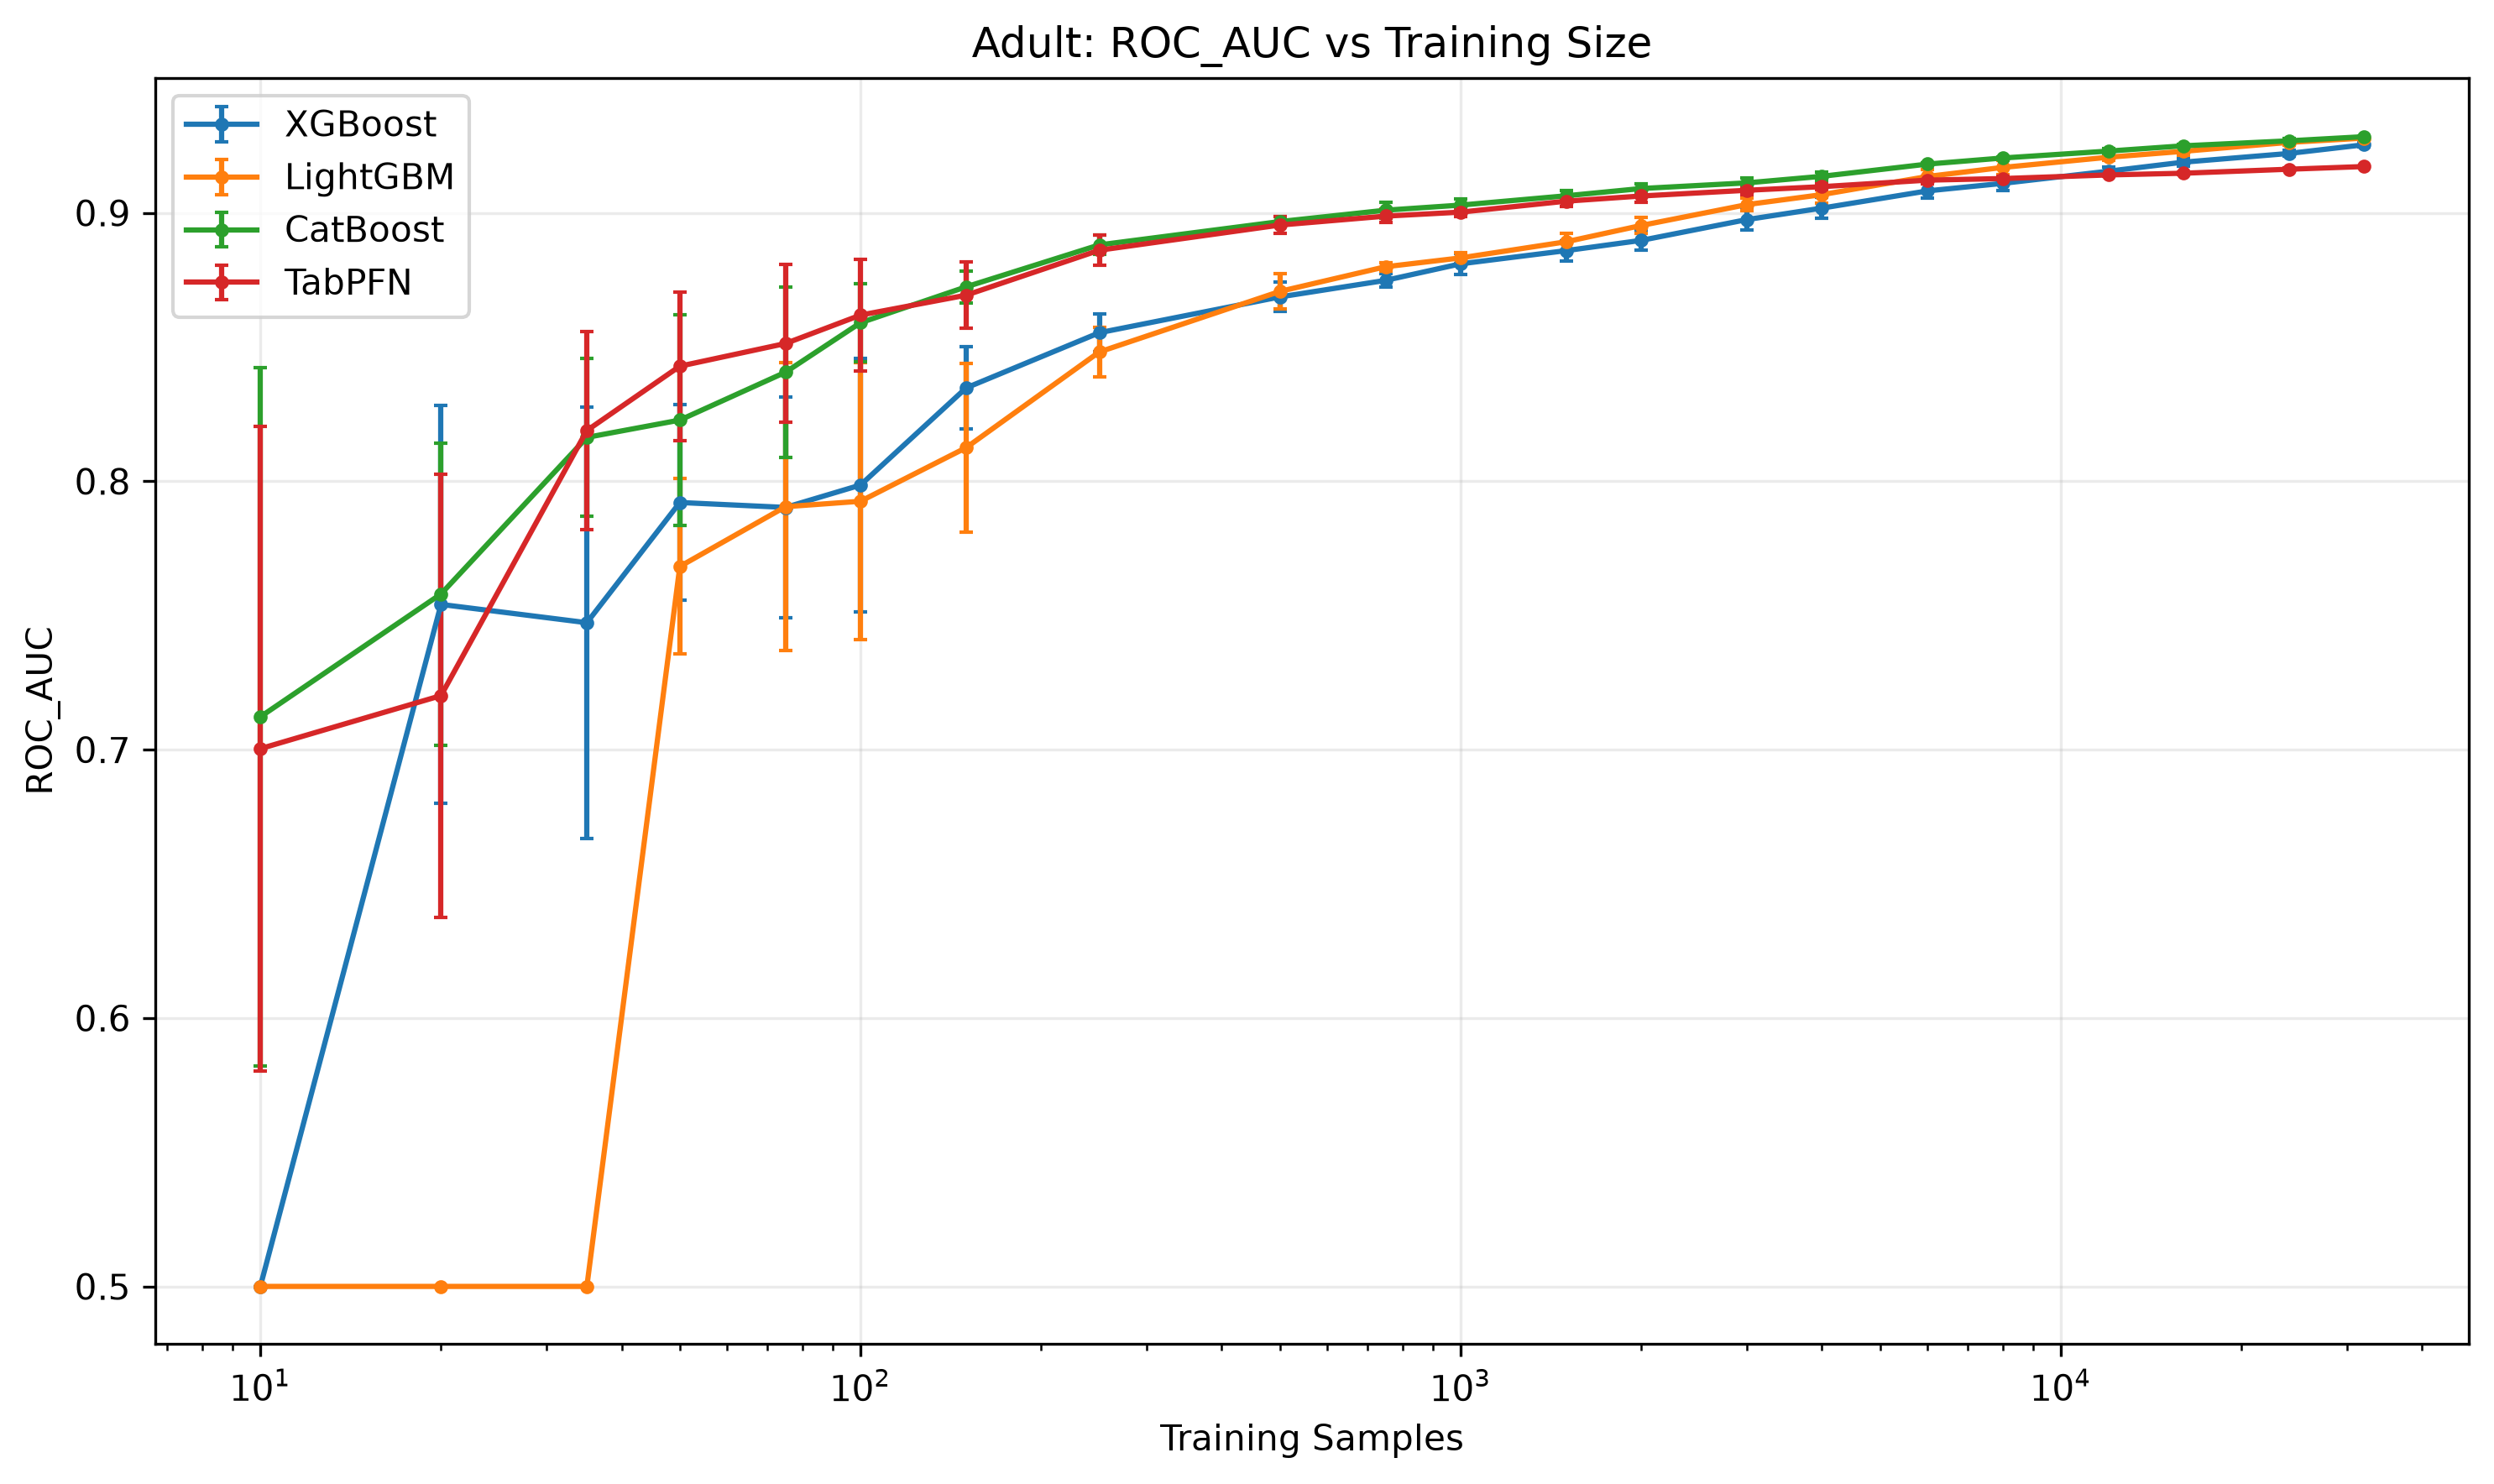
\includegraphics[width=\linewidth]{figures/adult_roc_auc_learning_curve.png}
  \caption{Adult ROC-AUC learning curve.}
  \label{fig:adult-roc-auc}
\end{figure}

\begin{figure}[htbp]
  \centering
  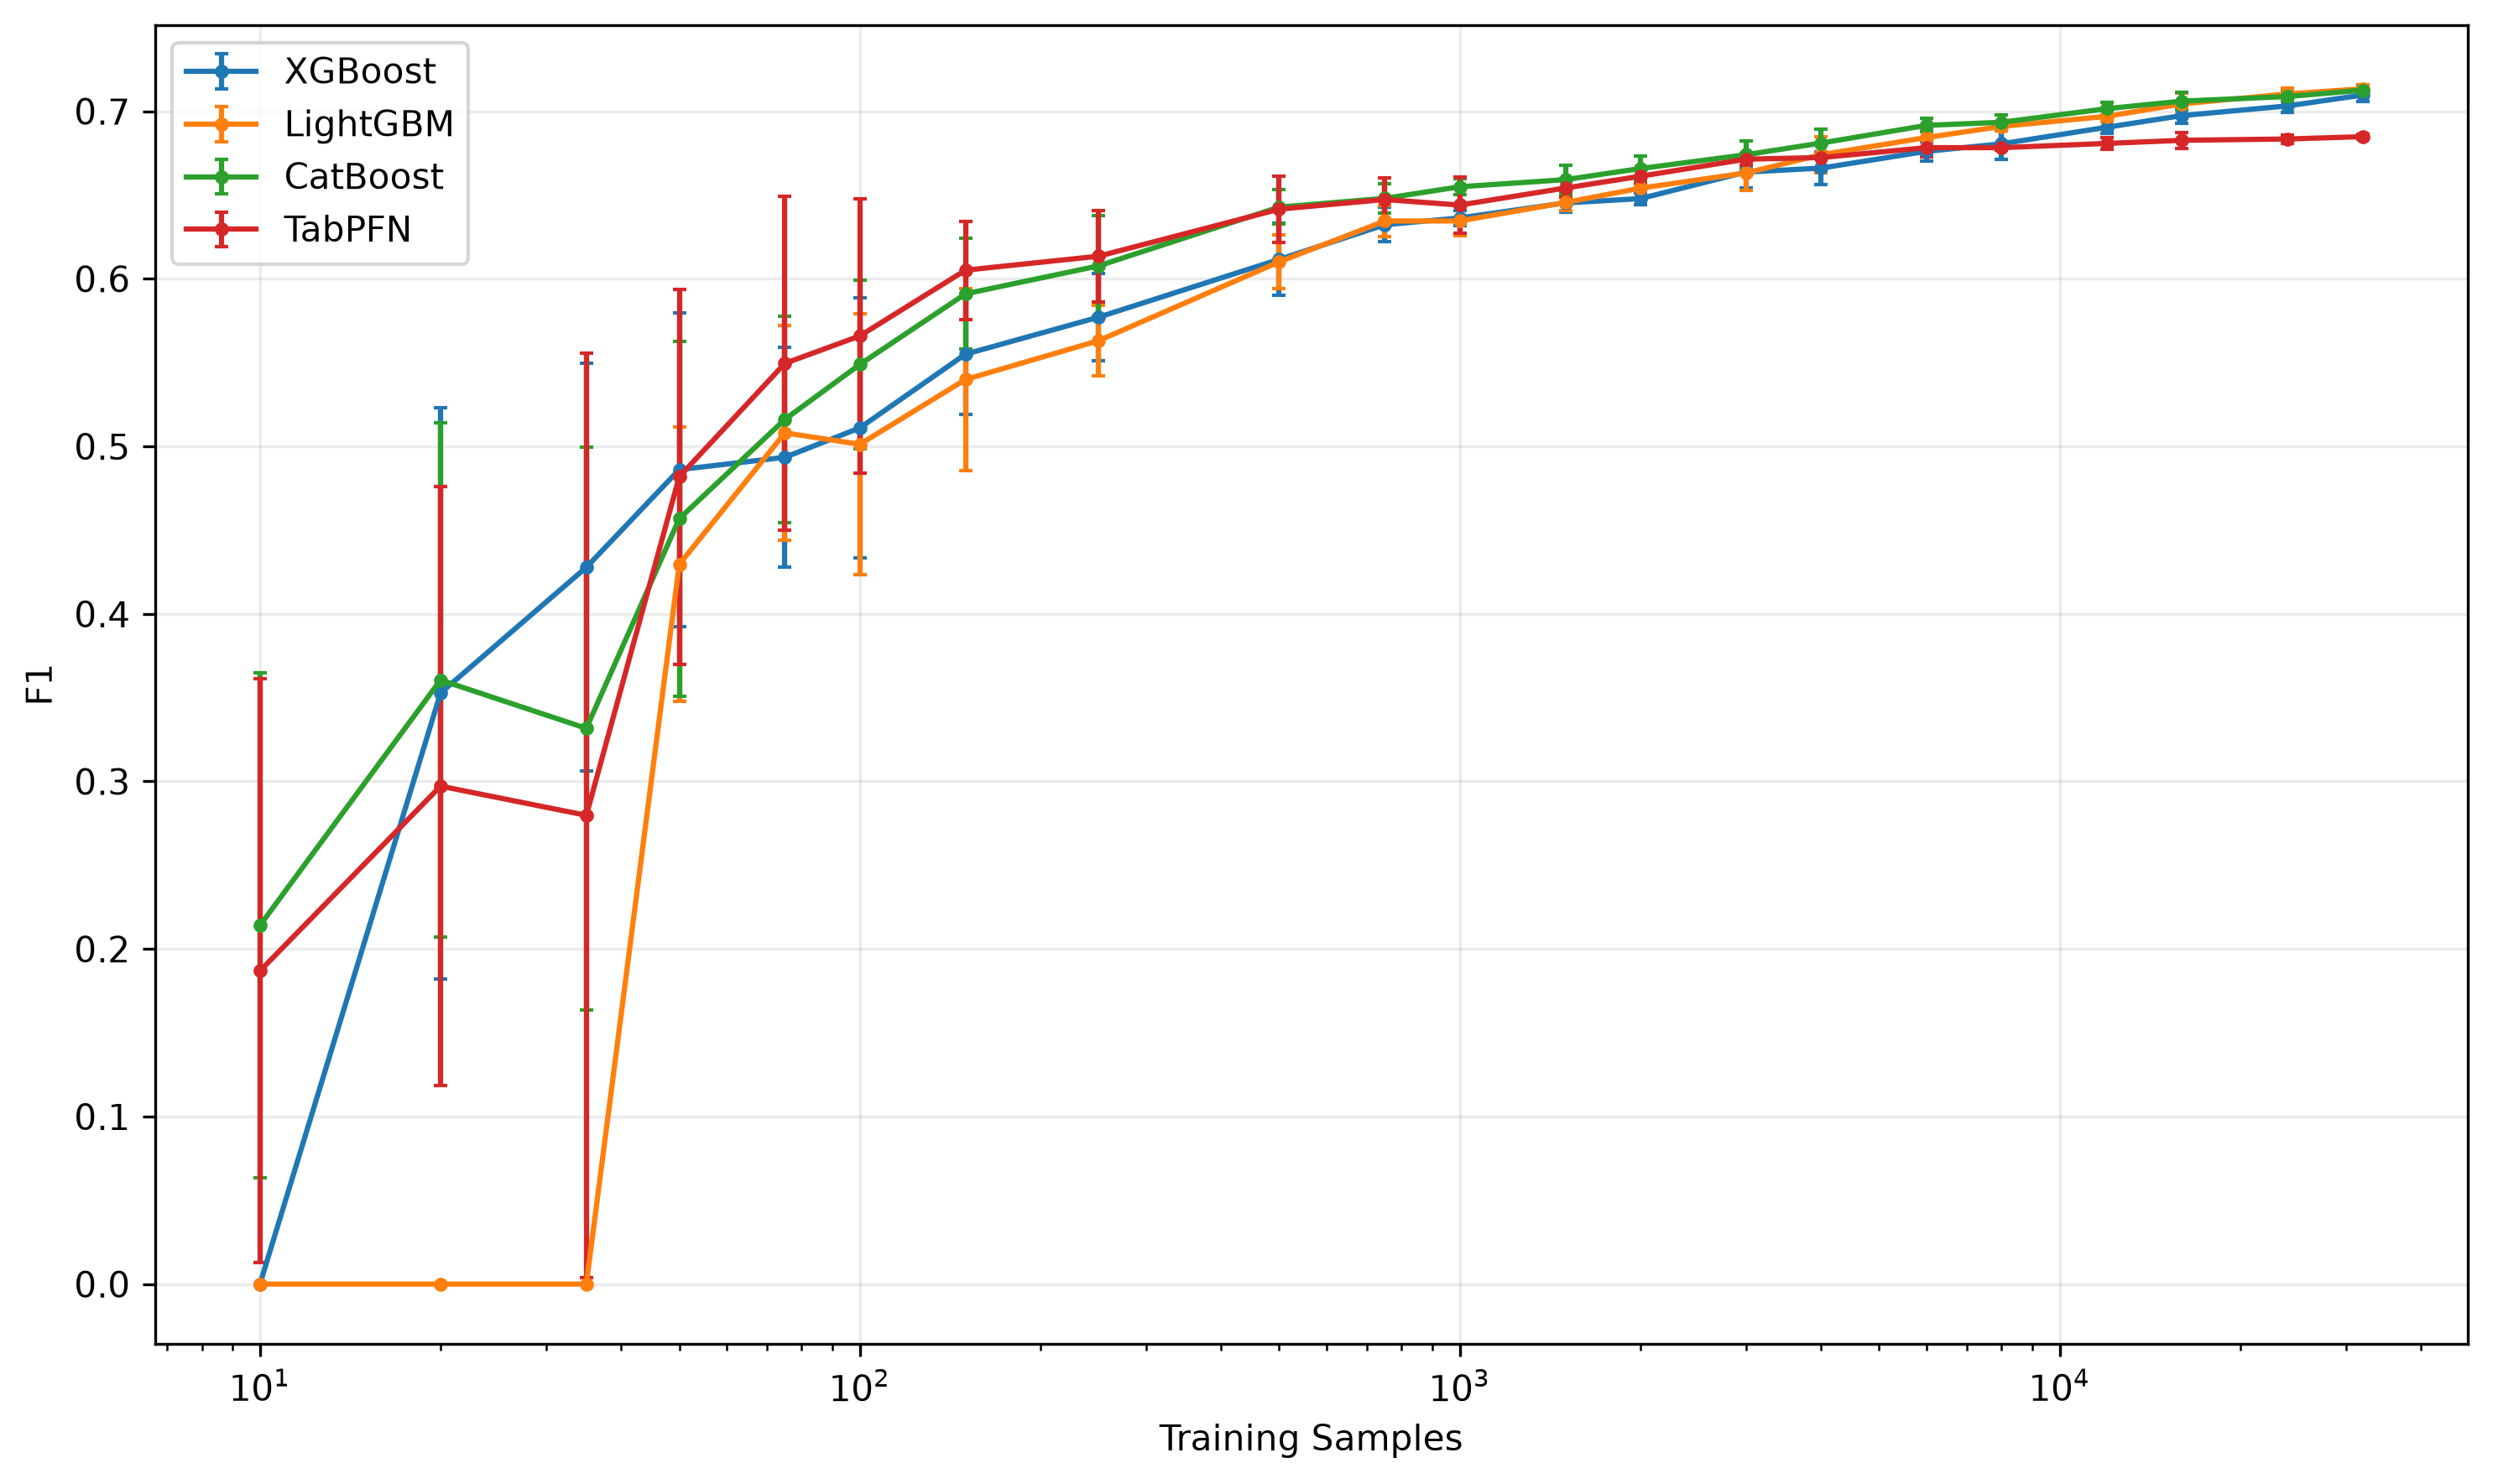
\includegraphics[width=\linewidth]{figures/adult_f1_learning_curve.png}
  \caption{Adult F1 learning curve.}
  \label{fig:adult-f1}
\end{figure}

\begin{figure}[htbp]
  \centering
  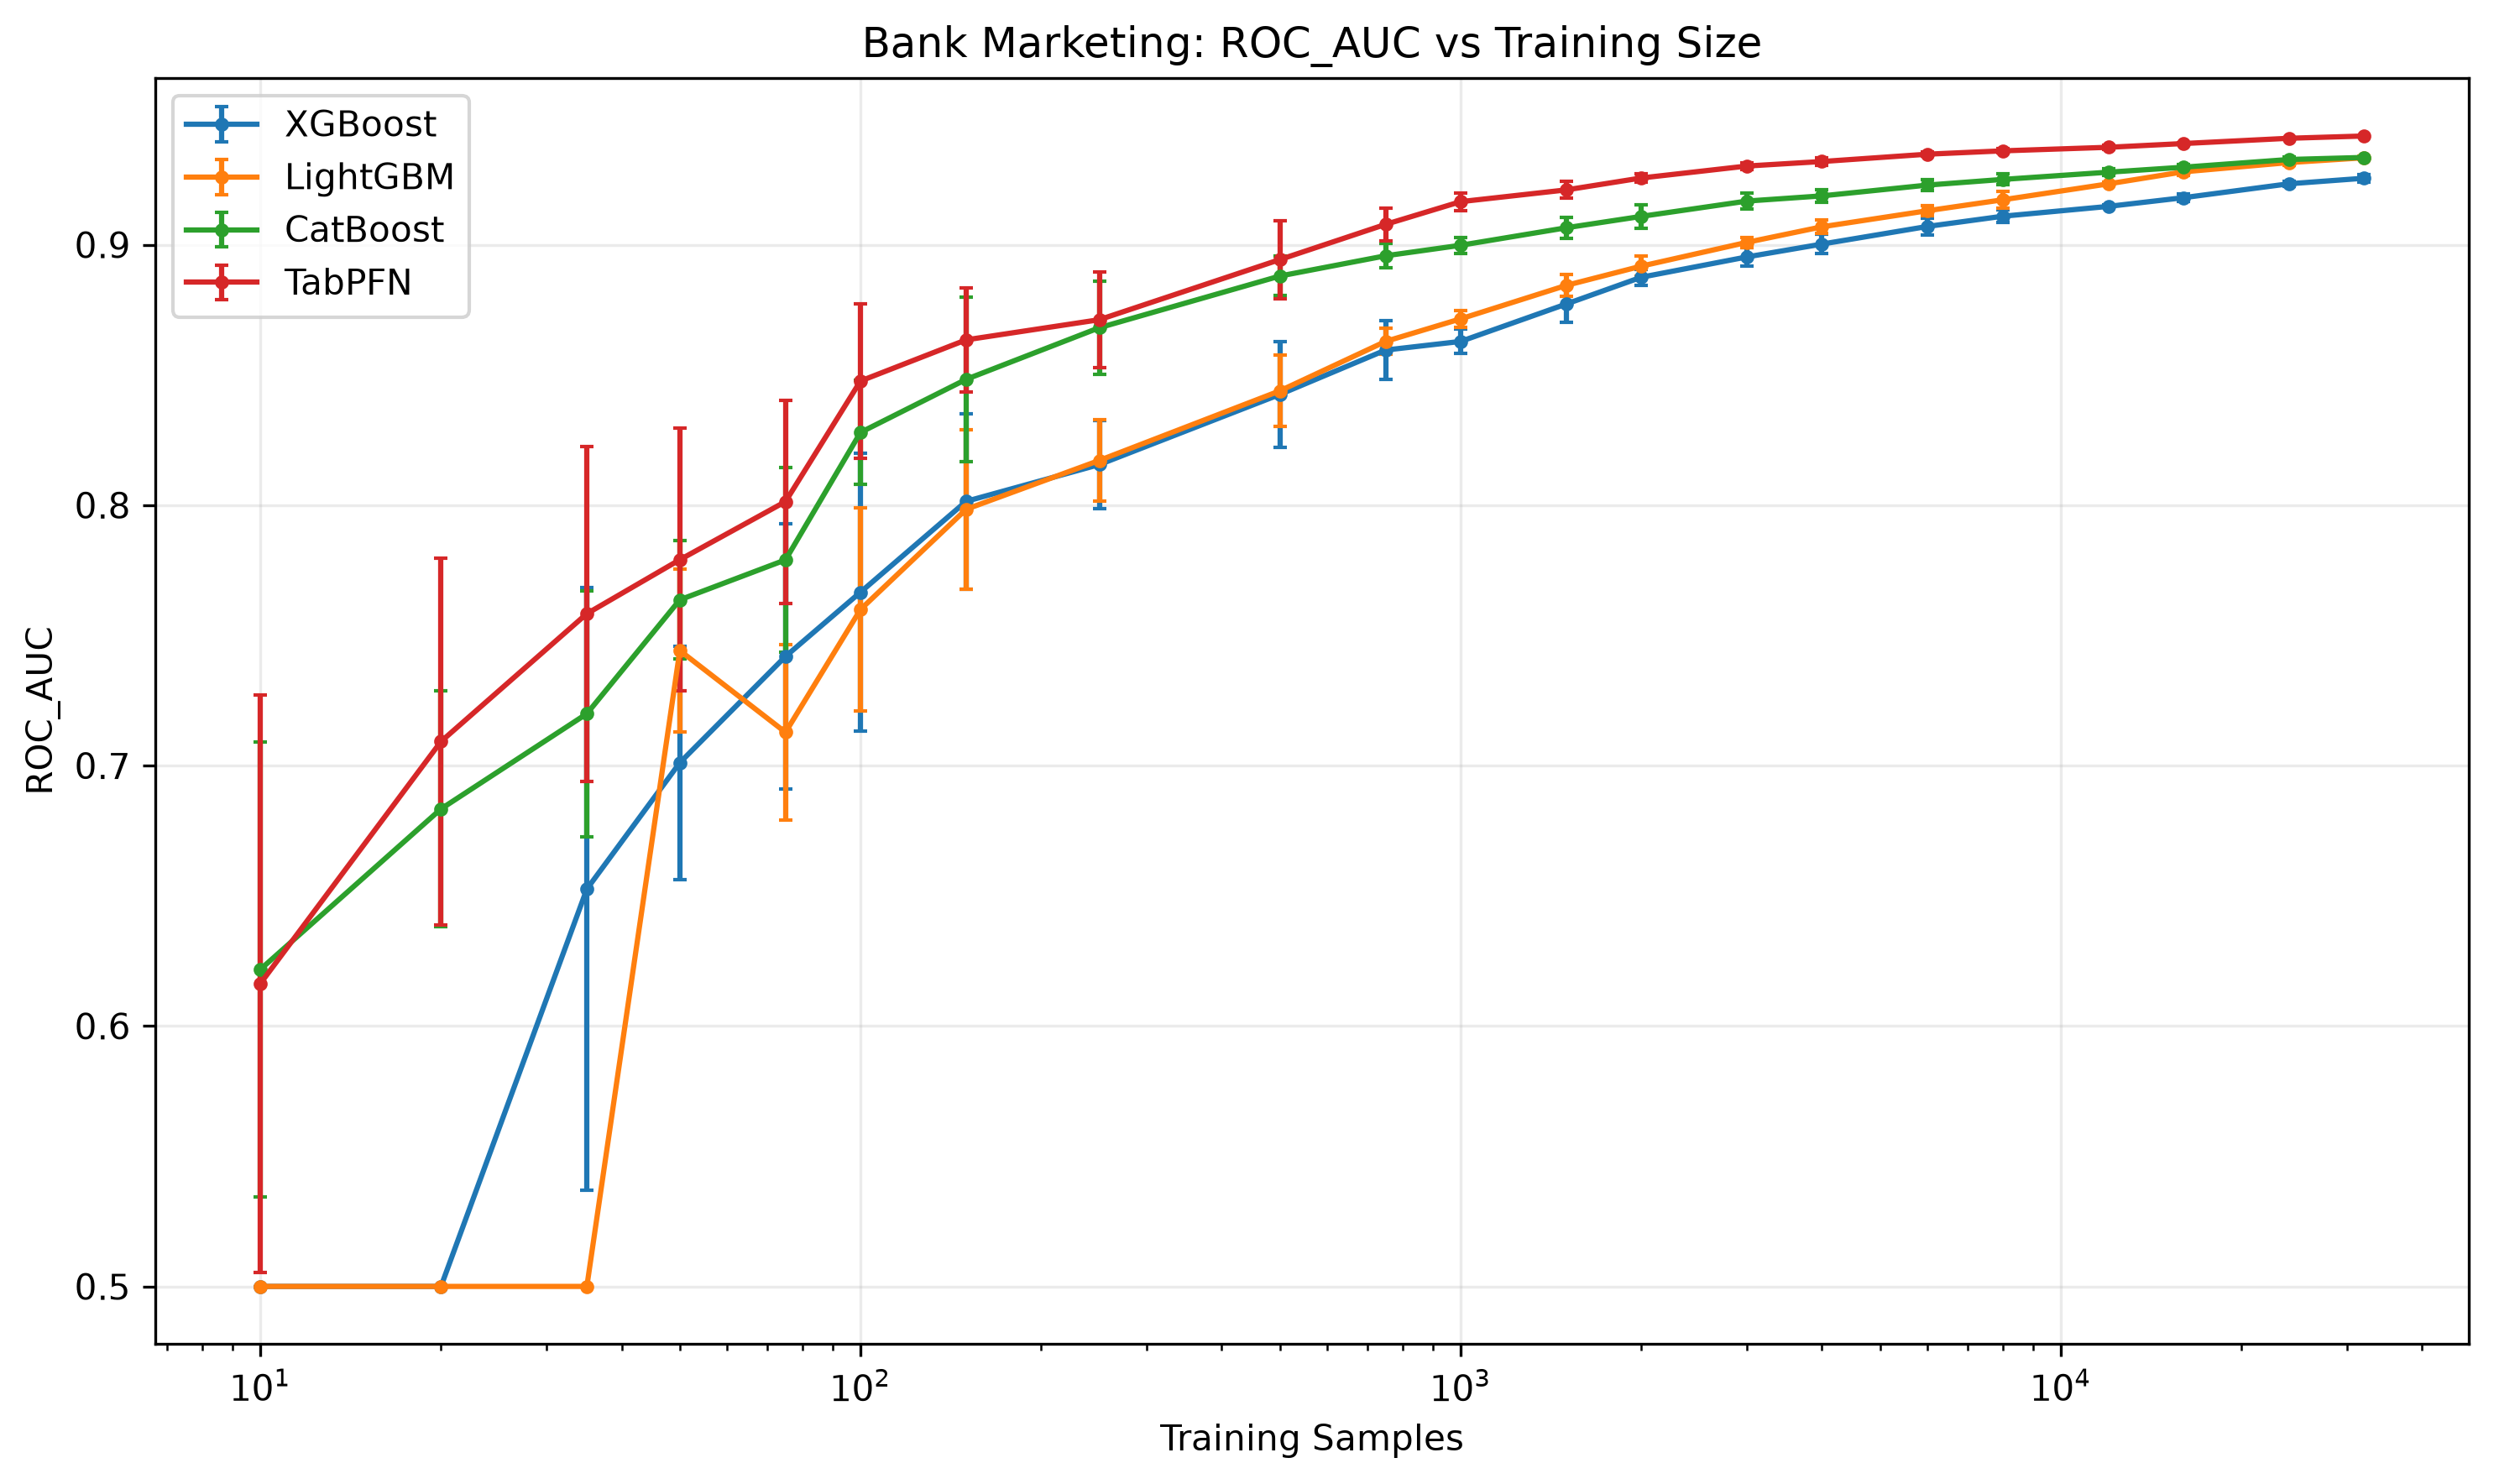
\includegraphics[width=\linewidth]{figures/bank_marketing_roc_auc_learning_curve.png}
  \caption{Bank Marketing ROC-AUC learning curve.}
  \label{fig:bank-roc-auc}
\end{figure}

\begin{figure}[htbp]
  \centering
  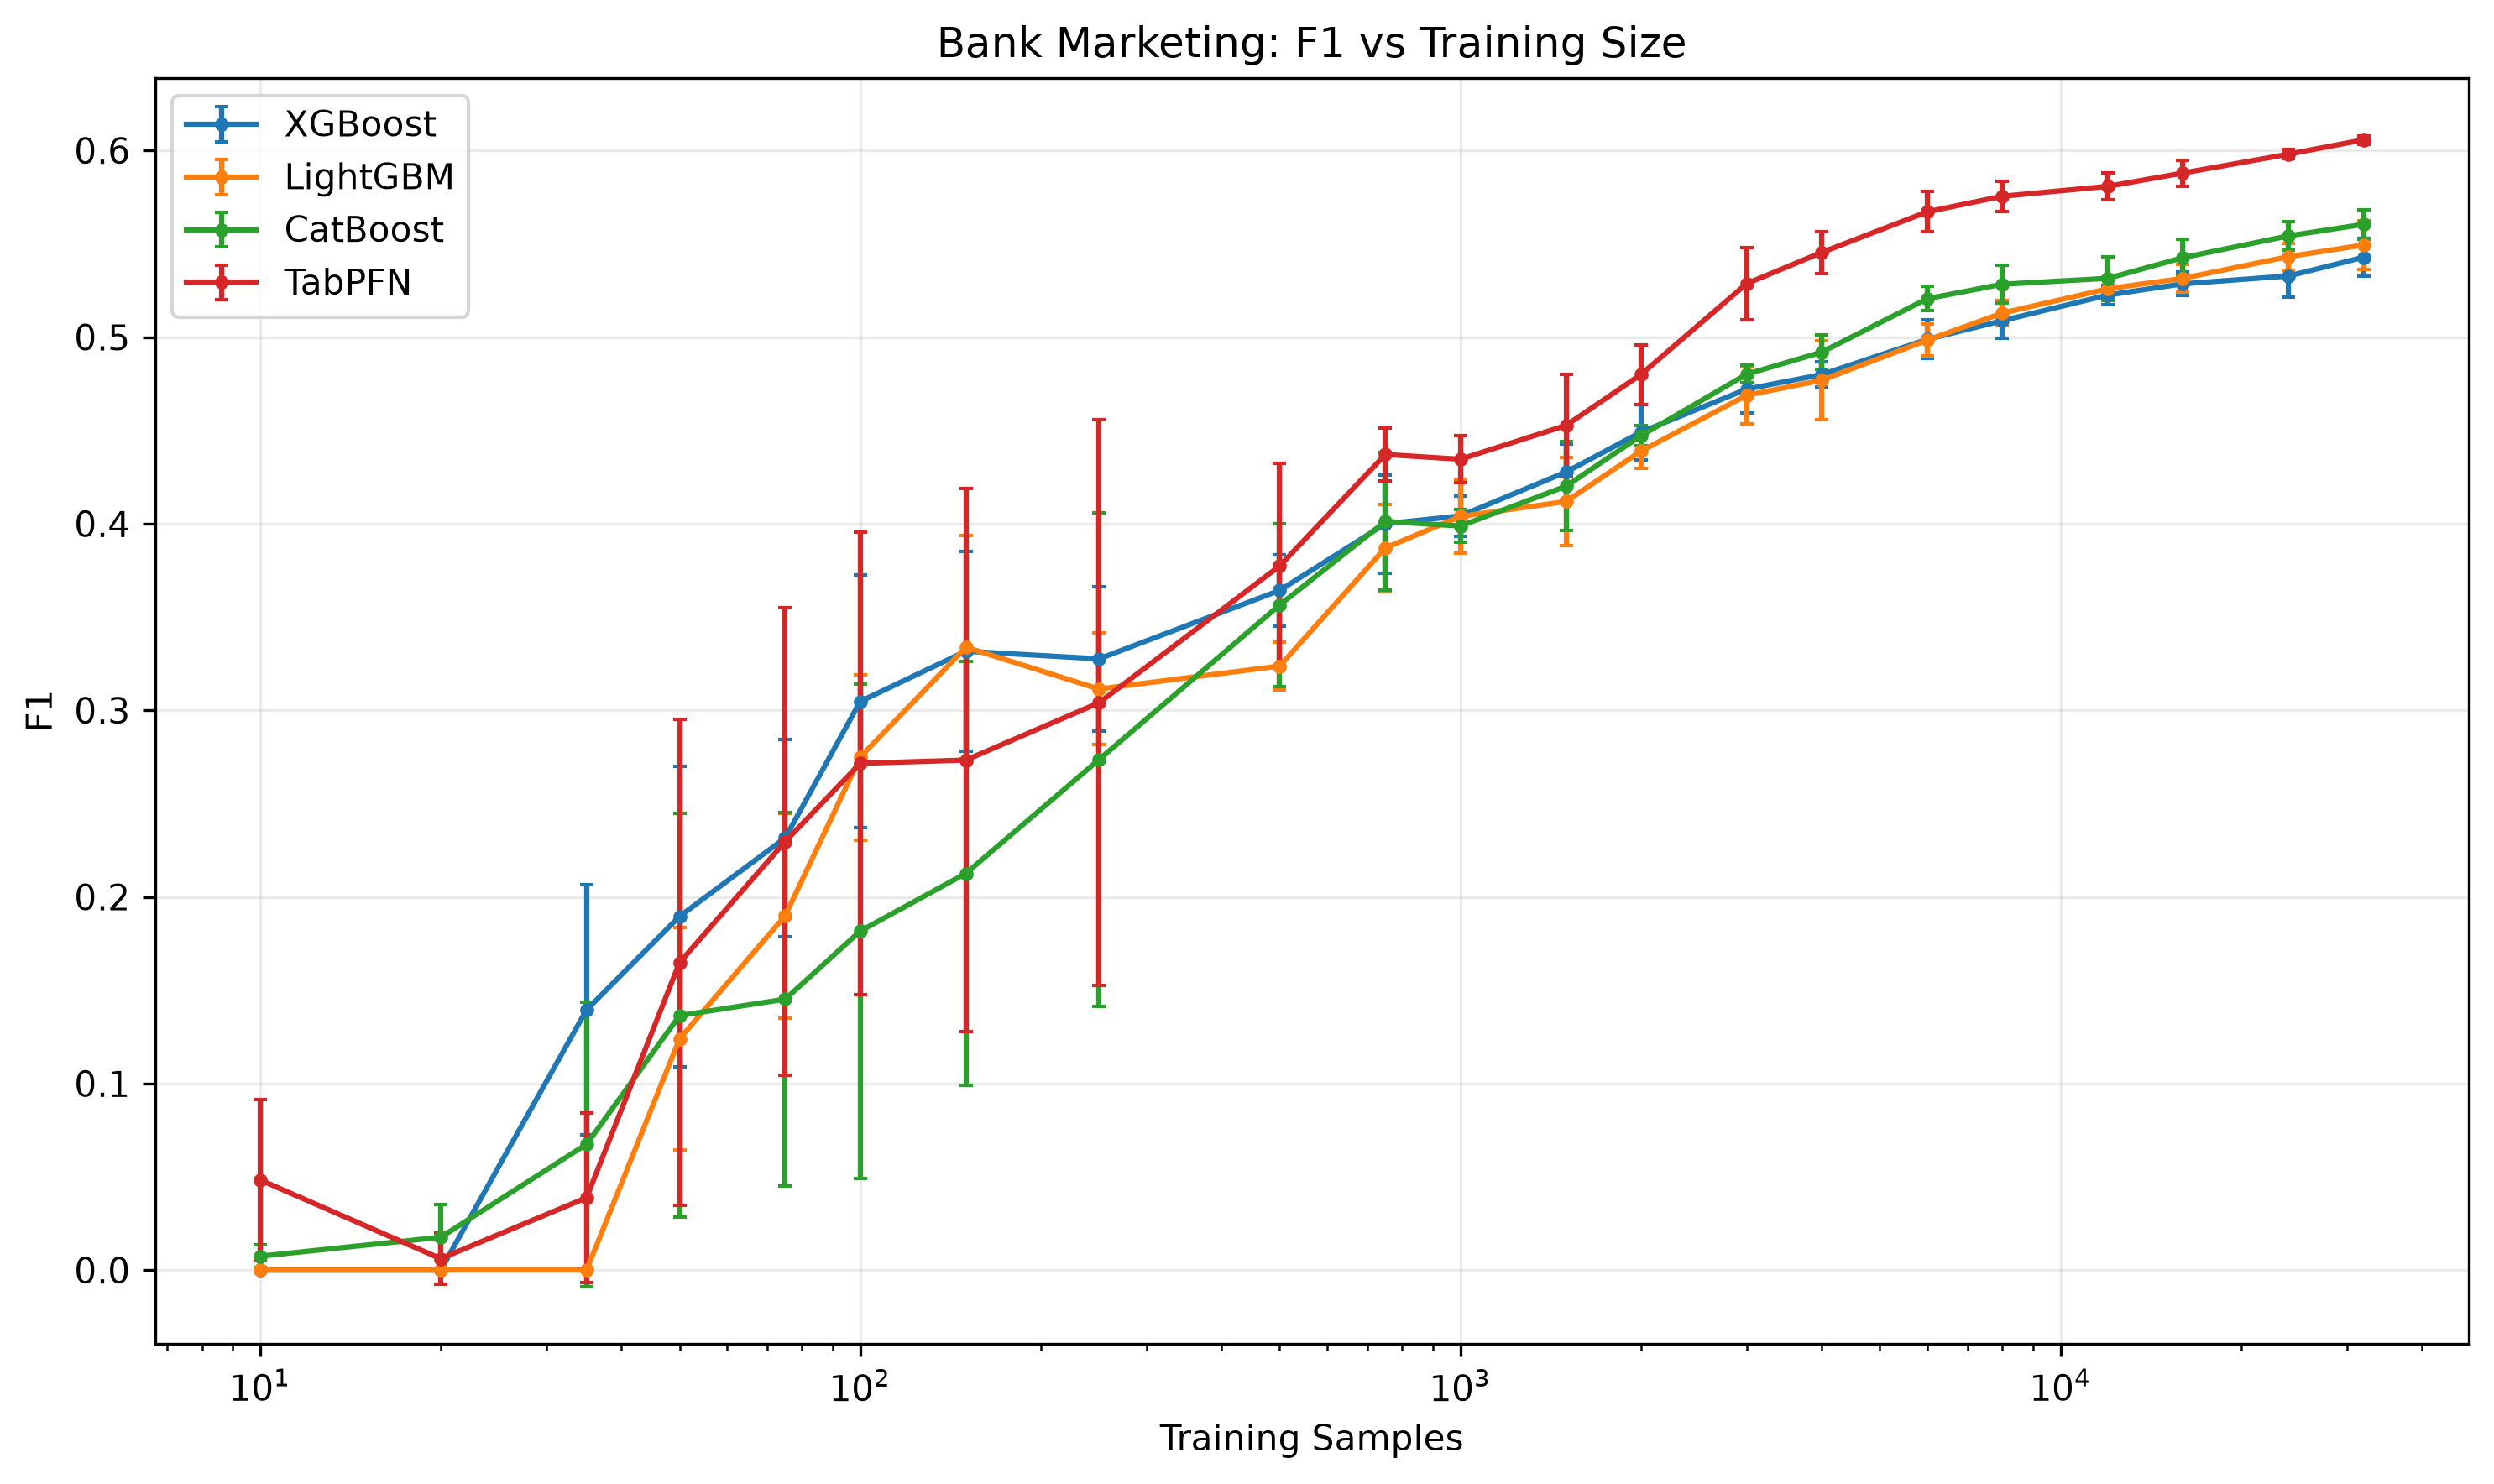
\includegraphics[width=\linewidth]{figures/bank_marketing_f1_learning_curve.png}
  \caption{Bank Marketing F1 learning curve.}
  \label{fig:bank-f1}
\end{figure}

\begin{figure}[htbp]
  \centering
  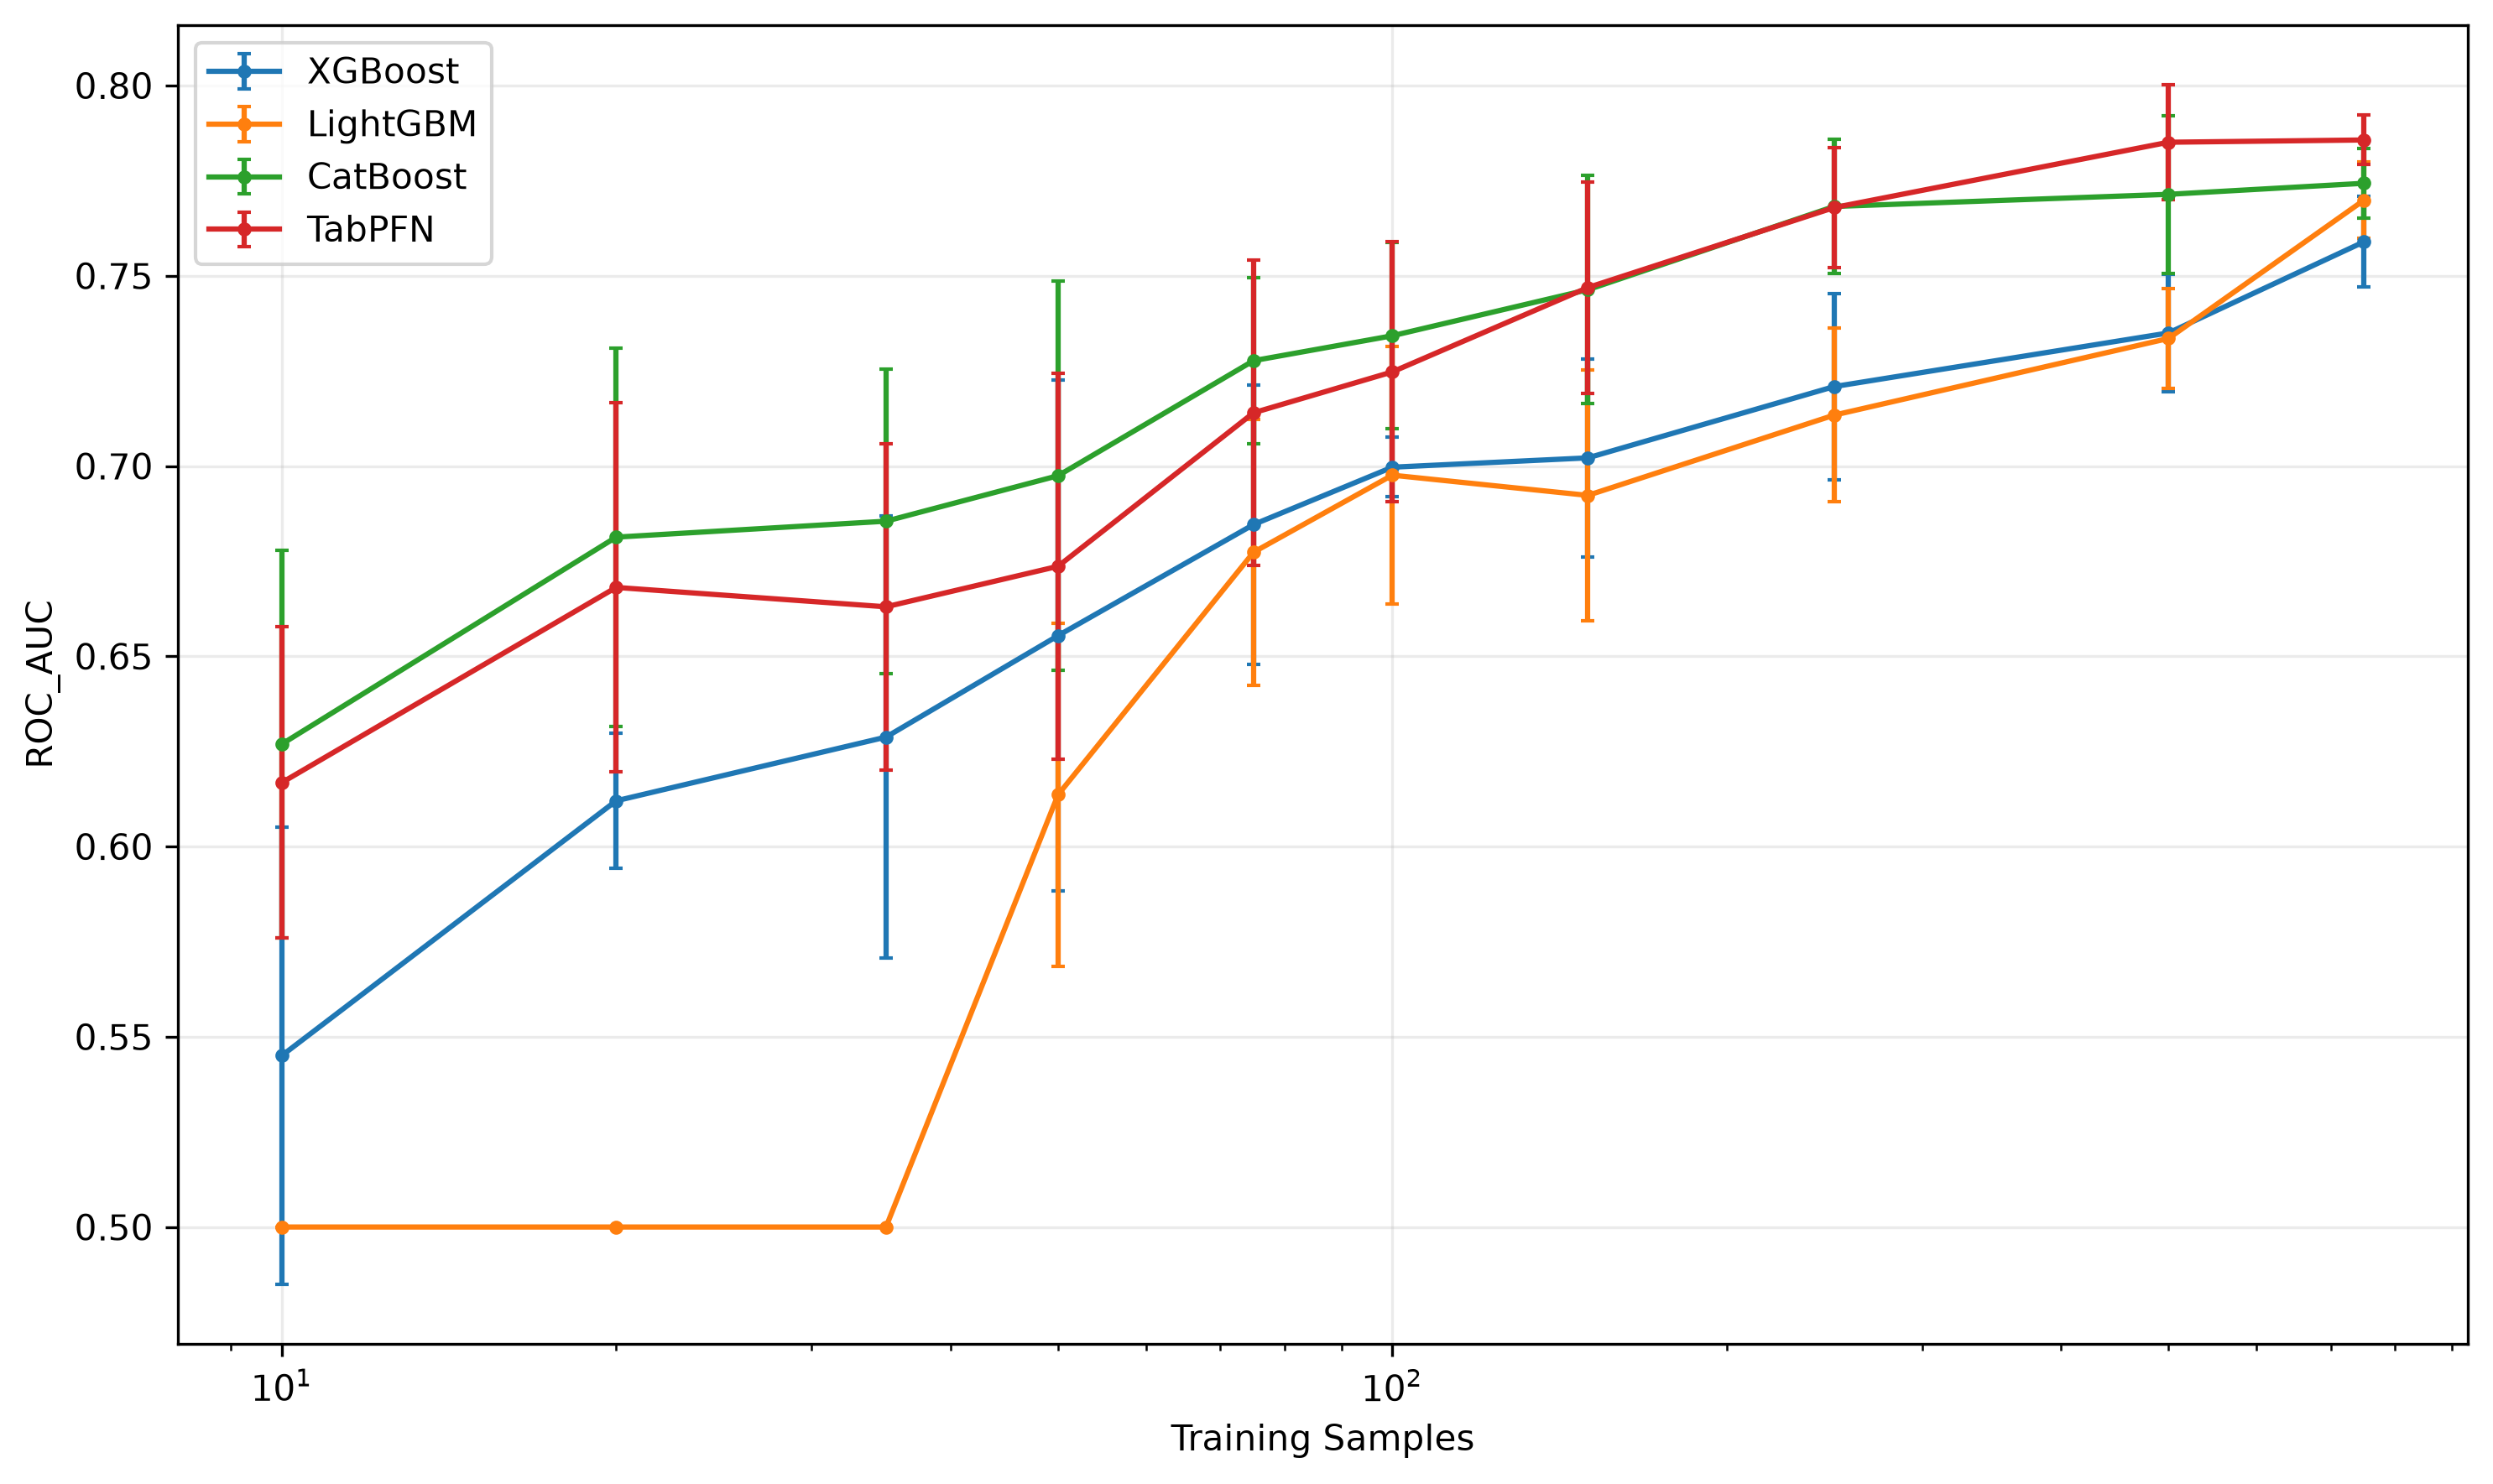
\includegraphics[width=\linewidth]{figures/credit-g_roc_auc_learning_curve.png}
  \caption{Credit-G ROC-AUC learning curve.}
  \label{fig:credit-roc-auc}
\end{figure}

\begin{figure}[htbp]
  \centering
  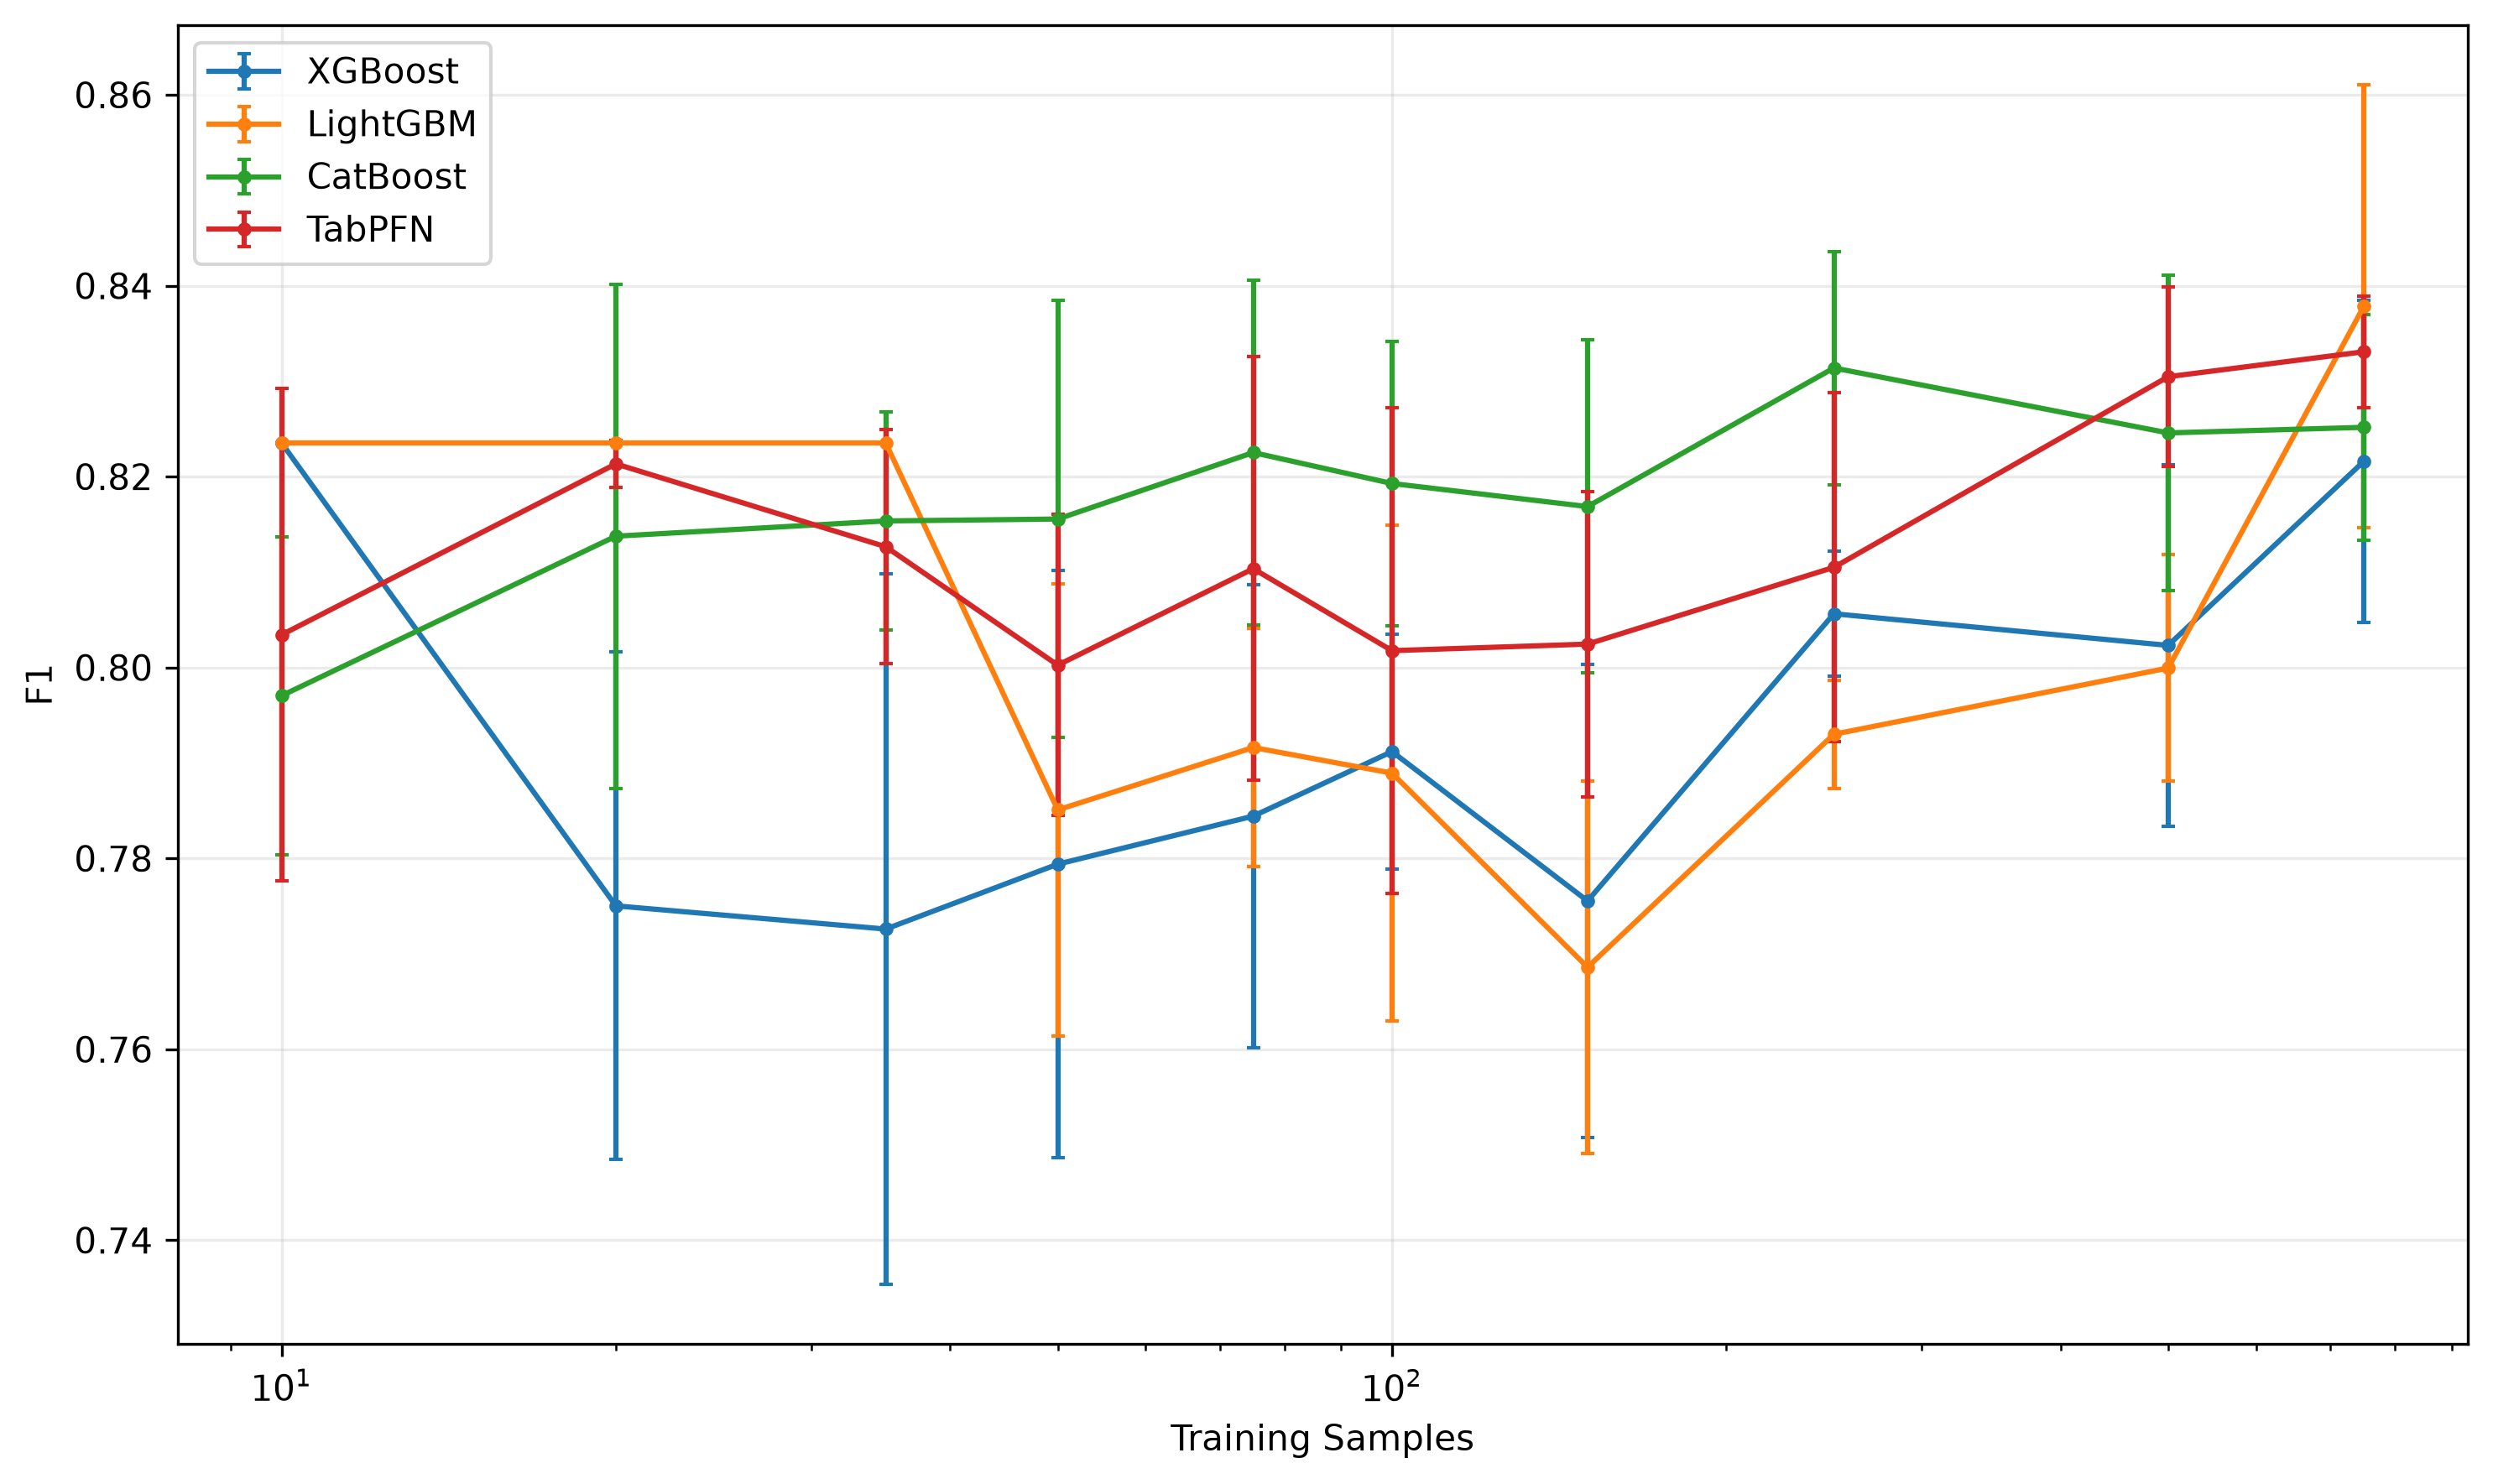
\includegraphics[width=\linewidth]{figures/credit-g_f1_learning_curve.png}
  \caption{Credit-G F1 learning curve.}
  \label{fig:credit-f1}
\end{figure}
